
\documentclass[a4paper]{article}

\usepackage[UTF8]{ctex}
\usepackage[a4paper,margin=1in]{geometry}
\usepackage{graphicx}
\usepackage{float}
\usepackage{listings}
\usepackage{longtable}
\usepackage{booktabs}
\usepackage{hyperref}
\usepackage{fancyhdr}
\usepackage{lastpage}
\usepackage{color}
\usepackage{indentfirst}        % 首段缩进
\setlength{\parindent}{2em}     % 缩进2字符
\usepackage{zhnumber}           % 中文编号
\usepackage[dvipsnames]{xcolor}
\usepackage{amsmath}            % 数学公式

%\newcommand{\college}{中山大学计算机学院}
\newcommand{\projname}{大数据实验 | Lab7}
\newcommand{\reporttitle}{混合推荐系统设计}
\newcommand{\stuno}{23336179}
\newcommand{\authorname}{马福泉}
\newcommand{\major}{计算机科学与技术}
\newcommand{\adviser}{王昌栋}
\newcommand{\startdate}{2026年4月21日}
\newcommand{\labenddate}{2026年4月23日}
\newcommand{\labroom}{B201}

\pagestyle{fancy} % 使用 fancyhdr 风格
\fancyhf{}      % 清空默认的页眉页脚

% 设置页眉
\fancyhead[L]{\kaishu \projname}      % 左侧页眉显示项目名称
\fancyhead[C]{\kaishu \reporttitle}    % 中间页眉显示报告标题
\fancyhead[R]{\kaishu \authorname} % 右侧页眉显示作者姓名

% 设置页脚
\fancyfoot[C]{第 \thepage 页，共 \pageref{LastPage} 页} % 中间页脚显示页码

% 去除页眉页脚与正文之间的分隔线
\renewcommand{\headrulewidth}{0.4pt}
\renewcommand{\footrulewidth}{0pt}

% 设置文档背景颜色
\definecolor{mybgcolor}{RGB}{0, 0, 0} % 定义背景颜色
\definecolor{NavyBlue}{RGB}{0,0,128} % 添加颜色定义
% \pagecolor{mybgcolor} % 设置背景颜色

% listing 配置python（美观样式）
\definecolor{codegreen}{RGB}{0,128,0}
\definecolor{codegray}{RGB}{128,128,128}
\definecolor{codepurple}{RGB}{128,0,128}
\definecolor{codeblue}{RGB}{0,0,255}
\definecolor{codeorange}{RGB}{255,128,0}

\lstset{
    language=Python,
    basicstyle=\ttfamily\footnotesize,
    keywordstyle=\color{codeblue}\bfseries,
    commentstyle=\color{codegreen}\itshape,
    stringstyle=\color{codepurple},
    numbers=left,
    numberstyle=\tiny\color{codegray},
    stepnumber=1,
    numbersep=5pt,
    backgroundcolor=\color{white},
    showspaces=false,
    showstringspaces=false,
    showtabs=false,
    frame=single,
    tabsize=4,
    captionpos=b,
    breaklines=true,
    breakatwhitespace=false,
    escapeinside={\%*}{*)},
    morekeywords={self, True, False, None, as, with, yield, lambda, assert, raise, except, finally, import, from, pandas, numpy, pd, np, sklearn, fit, predict, recommend, DataFrame, Series, defaultdict, cosine_similarity, TfidfVectorizer}
}

\begin{document}

% 封面
\begin{titlepage}
    \centering
    

    
\includegraphics[width=10cm]{img/SYSULogo.png}

    \vspace{1em}
    %{\Large \college \par}
    \vspace{1em}
    {\Large \kaishu \projname \par}
    \vspace{3em}

    

    
    {\fontsize{40pt}{42pt}\kaishu \selectfont \boldmath \reporttitle\par}
    \vspace*{\fill}

    \begin{center}
    {\Large
    \makebox[5em][s]{学号}:\underline{\makebox[15em][c]{\kaishu \stuno}}\\[1em]
    \makebox[5em][s]{姓名}:\underline{\makebox[15em][c]{\kaishu \authorname}}\\[1em]
    \makebox[5em][s]{专业}:\underline{\makebox[15em][c]{\kaishu \major}}\\[1em]
    \makebox[5em][s]{指导教师}:\underline{\makebox[15em][c]{\kaishu \adviser}}\\[1em]
    \makebox[5em][s]{起始日期}:\underline{\makebox[15em][c]{\kaishu \startdate}}\\[1em]
    \makebox[5em][s]{结束日期}:\underline{\makebox[15em][c]{\kaishu \labenddate}}\\[1em]
    \makebox[5em][s]{实验地点}:\underline{\makebox[15em][c]{\kaishu \labroom}}
    }
    \end{center}

    \vspace*{\fill}
\end{titlepage}

% 目录
\tableofcontents
\newpage

\section{实验要求}

本次实验为Lab7：混合推荐系统设计。实验要求如下：

\begin{enumerate}
    \item 基于MovieLens数据集。
    \item 实现协同过滤（用户/物品相似度）与基于内容的推荐（电影标签），对比两者召回率。
    \item （可选）设计加权混合策略或其他策略提升推荐多样性。
\end{enumerate}
\section{分析设计}

\subsection{实验说明}

\subsubsection{实验环境}

本实验软件环境如下：

\begin{itemize}
    \item \textbf{Python版本}: Python 3.8 或以上版本
    \item \textbf{核心依赖库}:
    \begin{itemize}
        \item \texttt{pandas}: 数据处理与分析，用于加载和处理MovieLens数据集
        \item \texttt{numpy}: 数值计算，用于矩阵运算和相似度计算
        \item \texttt{scikit-learn}: 机器学习库，提供TF-IDF向量化、余弦相似度计算等功能
        \item \texttt{matplotlib}: 数据可视化，用于生成评估指标对比图表
        \item \texttt{seaborn}: 统计数据可视化，辅助图表美化
    \end{itemize}
    \item \textbf{开发环境}: 使用虚拟环境（venv）隔离项目依赖
\end{itemize}

\subsubsection{文件架构}

本实验项目的文件夹树状结构如下：

项目文件结构如下：

\begin{itemize}
    \item \textbf{lab7/} --- 项目根目录
    \begin{itemize}
        \item \textbf{data/} --- MovieLens数据集目录
        \begin{itemize}
            \item \texttt{movies.csv} --- 电影信息（movieId, title, genres）
            \item \texttt{ratings.csv} --- 用户评分数据
            \item \texttt{tags.csv} --- 用户标签数据
            \item \texttt{links.csv} --- 外部链接ID
            \item \texttt{README.txt} --- 数据集说明文档
        \end{itemize}
        \item \textbf{src/} --- Python源代码目录
        \begin{itemize}
            \item \texttt{result.txt} --- 实验结果输出文件
            \item \texttt{data\_loader.py} --- 数据加载与预处理模块
            \item \texttt{collaborative\_filtering.py} --- 协同过滤算法实现
            \item \texttt{content\_based.py} --- 基于内容推荐算法实现
            \item \texttt{hybrid\_recommender.py} --- 混合推荐策略实现
            \item \texttt{evaluation.py} --- 评估指标计算模块
            \item \texttt{visualization.py} --- 可视化图表生成模块
            \item \texttt{main.py} --- 主程序入口
        \end{itemize}
        \item \textbf{img/} --- 可视化图表输出目录
        \begin{itemize}
            \item \texttt{SYSULogo.png} --- 中山大学校徽（报告封面）
            \item \texttt{recall\_comparison.png} --- 召回率对比图
            \item \texttt{coverage\_comparison.png} --- 覆盖率对比图
            \item \texttt{diversity\_comparison.png} --- 多样性对比图
            \item 其他评估图表...
        \end{itemize}
        \item \textbf{lab7.tex} --- LaTeX实验报告源文件
        \item \textbf{lab7.pdf} --- LaTeX实验报告PDF
        \item \textbf{.venv/} --- Python虚拟环境（需手动创建）
    \end{itemize}
\end{itemize}

\subsection{数据集预处理设计}
数据预处理流程如下：
\begin{enumerate}
    \item 加载原始CSV文件并构建数据结构。
    \item 按用户划分训练集和测试集（80\%/20\%比例），确保每个用户都有训练和测试数据。
    \item 构建用户-电影评分矩阵（User-Item Matrix）。
    \item 提取电影特征（类型genres和标签tags）用于基于内容的推荐。
\end{enumerate}

\subsection{协同过滤算法设计}

协同过滤（Collaborative Filtering, CF）是推荐系统中最经典的算法之一。本实验实现基于用户的协同过滤（User-based CF）。

\subsubsection{核心思想}

基于用户的协同过滤假设：如果两个用户在过去对物品的评分行为相似，那么他们对未来物品的评分也会相似。算法流程如下：
\begin{enumerate}
    \item 计算目标用户与其他用户的相似度。
    \item 选择相似度最高的$k$个用户作为邻居。
    \item 根据邻居的评分预测目标用户对未评分物品的评分。
    \item 推荐预测评分最高的物品。
\end{enumerate}

\subsubsection{相似度计算}

本实验使用\textbf{余弦相似度}（Cosine Similarity）计算用户相似度：

\begin{equation}
\text{sim}(u, v) = \frac{\sum_{i \in I_{uv}} r_{ui} \cdot r_{vi}}{\sqrt{\sum_{i \in I_u} r_{ui}^2} \cdot \sqrt{\sum_{i \in I_v} r_{vi}^2}}
\end{equation}

其中，$I_{uv}$表示用户$u$和$v$共同评分过的物品集合，$r_{ui}$表示用户$u$对物品$i$的评分。

评分预测采用加权平均方法：

\begin{equation}
\hat{r}_{ui} = \bar{r}_u + \frac{\sum_{v \in N(u)} \text{sim}(u, v) \cdot (r_{vi} - \bar{r}_v)}{\sum_{v \in N(u)} |\text{sim}(u, v)|}
\end{equation}

其中，$\bar{r}_u$表示用户$u$的平均评分，$N(u)$表示用户$u$的邻居集合。

\subsection{基于内容推荐算法设计}

基于内容的推荐（Content-Based, CB）通过分析物品的内容特征来推荐与用户历史偏好相似的物品。

\subsubsection{核心思想}

本实验利用电影的类型（genres）和用户标签（tags）作为内容特征：
\begin{enumerate}
    \item 将每部电影的类型和标签合并为文本描述。
    \item 使用TF-IDF技术将文本转化为特征向量。
    \item 构建用户画像：用户已评分电影特征向量的加权平均。
    \item 计算用户画像与候选电影的相似度进行推荐。
\end{enumerate}

\subsubsection{TF-IDF特征提取}

TF-IDF（Term Frequency-Inverse Document Frequency）是一种常用的文本特征提取方法：

\begin{equation}
\text{TF-IDF}(t, d) = \text{TF}(t, d) \cdot \text{IDF}(t)
\end{equation}

\begin{equation}
\text{TF}(t, d) = \frac{f_{t,d}}{\sum_{t' \in d} f_{t',d}}
\end{equation}

\begin{equation}
\text{IDF}(t) = \log \frac{N}{|\{d \in D : t \in d\}|}
\end{equation}

其中，$f_{t,d}$表示词$t$在文档$d$中的出现频率，$N$表示文档总数。

\subsubsection{用户画像构建}

用户画像表示用户的偏好特征向量：

\begin{equation}
\text{profile}(u) = \frac{\sum_{i \in I_u} (r_{ui} - \bar{r}) \cdot \text{tfidf}(i)}{\sum_{i \in I_u} |r_{ui} - \bar{r}|}
\end{equation}

其中，$\text{tfidf}(i)$表示电影$i$的TF-IDF特征向量，使用评分偏差作为权重。

\subsection{混合推荐策略设计}

混合推荐（Hybrid）结合CF和CB的优势，以提升推荐效果。本实验采用\textbf{加权混合策略}：

\begin{equation}
\hat{r}_{ui}^{\text{hybrid}} = w_{\text{CF}} \cdot \hat{r}_{ui}^{\text{CF}} + w_{\text{CB}} \cdot \hat{r}_{ui}^{\text{CB}}
\end{equation}

权重设置：$w_{\text{CF}} = 0.6$，$w_{\text{CB}} = 0.4$。

混合策略的优势：
\begin{itemize}
    \item CF能发现用户潜在兴趣，但存在冷启动问题。
    \item CB能处理新物品，但推荐结果较为保守。
    \item 混合策略结合两者优势，有望提升召回率和多样性。
\end{itemize}

\subsection{评估指标设计}

本实验采用以下评估指标：

\begin{enumerate}
    \item \textbf{召回率（Recall Rate）}: 推荐命中数 / 用户实际喜欢数
    \begin{equation}
    \text{Recall} = \frac{|\text{Recommended} \cap \text{Liked}|}{|\text{Liked}|}
    \end{equation}
    
    \item \textbf{精确率（Precision）}: 推荐命中数 / 推荐总数
    \begin{equation}
    \text{Precision} = \frac{|\text{Recommended} \cap \text{Liked}|}{|\text{Recommended}|}
    \end{equation}
    
    \item \textbf{覆盖率（Coverage）}: 被推荐电影数 / 总电影数
    \begin{equation}
    \text{Coverage} = \frac{|\cup_{u} R_u|}{|I|}
    \end{equation}
    
    \item \textbf{多样性（Diversity）}: 推荐列表中物品间的平均不相似度
    \begin{equation}
    \text{Diversity} = \frac{1}{|R|(|R|-1)} \sum_{i,j \in R, i \neq j} (1 - \text{sim}(i, j))
    \end{equation}
\end{enumerate}

\section{核心代码}

\subsection{数据加载模块}

数据加载模块负责加载MovieLens数据集并进行预处理:

\begin{lstlisting}
class DataLoader:
    """MovieLens数据加载器"""
    
    def load_data(self):
        """加载所有数据文件"""
        # 加载电影数据
        self.movies = pd.read_csv(f'{self.data_dir}movies.csv')
        # 加载评分数据
        self.ratings = pd.read_csv(f'{self.data_dir}ratings.csv')
        # 加载标签数据
        self.tags = pd.read_csv(f'{self.data_dir}tags.csv')
        # 数据预处理
        self._preprocess()
        return True
    
    def get_user_movie_matrix(self, data=None):
        """构建用户-电影评分矩阵"""
        matrix = data.pivot_table(
            index='userId', 
            columns='movieId', 
            values='rating'
        )
        return matrix
\end{lstlisting}

\subsection{协同过滤核心代码}

协同过滤算法的核心是相似度计算和评分预测：

\begin{lstlisting}
class CollaborativeFiltering:
    """基于用户的协同过滤推荐系统"""
    
    def fit(self, user_movie_matrix):
        """训练模型：计算用户相似度矩阵"""
        # 计算每个用户的平均评分
        self.user_mean = self.user_movie_matrix.mean(axis=1)
        # 填充NaN为0（未评分）
        matrix_filled = self.user_movie_matrix.fillna(0)
        # 计算用户相似度矩阵（使用余弦相似度）
        self.user_similarity = pd.DataFrame(
            cosine_similarity(matrix_filled),
            index=user_movie_matrix.index,
            columns=user_movie_matrix.index
        )
    
    def predict_rating(self, user_id, movie_id):
        """预测用户对电影的评分"""
        # 获取邻居用户
        neighbors = self._get_neighbors(user_id)
        # 计算加权平均评分
        weighted_sum = 0
        sim_sum = 0
        for neighbor_id, sim in neighbors.items():
            neighbor_rating = self.user_movie_matrix.loc[neighbor_id, movie_id]
            if not np.isnan(neighbor_rating):
                neighbor_mean = self.user_mean.get(neighbor_id, 3.0)
                weighted_sum += (neighbor_rating - neighbor_mean) * sim
                sim_sum += abs(sim)
        # 返回预测评分
        return user_mean + weighted_sum / sim_sum
\end{lstlisting}

\subsection{基于内容推荐核心代码}

基于内容推荐使用TF-IDF提取电影特征：

\begin{lstlisting}
class ContentBasedRecommender:
    """基于内容的推荐系统"""
    
    def fit(self, movie_features, user_movie_matrix):
        """训练模型：构建TF-IDF特征矩阵"""
        # 准备电影内容文本
        documents = [movie_features[mid].get('combined', '') 
                     for mid in movie_ids]
        # 使用TF-IDF向量化
        self.tfidf_vectorizer = TfidfVectorizer(
            min_df=self.min_df,
            max_features=self.max_features,
            stop_words='english'
        )
        self.tfidf_matrix = self.tfidf_vectorizer.fit_transform(documents)
        # 计算电影相似度矩阵
        self.movie_similarity = cosine_similarity(self.tfidf_matrix)
        # 构建用户画像
        self._build_user_profiles()
    
    def _build_user_profiles(self):
        """构建用户画像"""
        for user_id in self.user_movie_matrix.index:
            user_ratings = self.user_movie_matrix.loc[user_id].dropna()
            # 计算加权特征向量
            weighted_vector = np.zeros(self.tfidf_matrix.shape[1])
            for movie_id, rating in user_ratings.items():
                idx = movie_id_to_idx[movie_id]
                weight = rating - 2.5  # 中心化
                weighted_vector += weight * self.tfidf_matrix[idx]
            self.user_profiles[user_id] = weighted_vector
\end{lstlisting}

\subsection{混合推荐核心代码}

混合推荐将CF和CB的预测评分加权组合：

\begin{lstlisting}
class HybridRecommender:
    """混合推荐系统"""
    
    def __init__(self, cf_weight=0.6, cb_weight=0.4):
        """初始化混合推荐模型"""
        # 归一化权重
        total = cf_weight + cb_weight
        self.cf_weight = cf_weight / total
        self.cb_weight = cb_weight / total
    
    def predict_rating(self, user_id, movie_id):
        """预测用户对电影的评分"""
        # 获取CF预测
        cf_score = self.cf_model.predict_rating(user_id, movie_id)
        # 获取CB预测
        cb_score = self.cb_model.predict_rating(user_id, movie_id)
        # 加权平均
        hybrid_score = self.cf_weight * cf_score + self.cb_weight * cb_score
        return hybrid_score
\end{lstlisting}

\subsection{评估模块核心代码}

评估模块计算召回率、覆盖率、多样性等指标：

\begin{lstlisting}
class RecommenderEvaluator:
    """推荐系统评估器"""
    
    def evaluate(self, recommender, train_matrix, test_data, 
                 movie_features=None, n_recommendations=10):
        """评估推荐系统"""
        # 构建测试集用户-电影映射
        test_user_movies = defaultdict(set)
        for _, row in test_data.iterrows():
            if row['rating'] >= self.rating_threshold:
                test_user_movies[row['userId']].add(row['movieId'])
        
        # 计算指标
        for user_id in test_users:
            recommendations = recommender.recommend(user_id, n_recommendations)
            recommended_movies = set([mid for mid, _ in recommendations])
            actual_movies = test_user_movies.get(user_id, set())
            # 计算命中数
            hits = len(recommended_movies & actual_movies)
            # 召回率
            recall = hits / len(actual_movies)
            # 精确率
            precision = hits / n_recommendations
        
        # 返回评估结果
        return {
            'recall': avg_recall,
            'precision': avg_precision,
            'coverage': coverage,
            'diversity': avg_diversity
        }
\end{lstlisting}

\section{结果分析}

\subsection{实验参数设置}

\begin{itemize}
    \item 数据集：MovieLens ml-latest-small（9742部电影，100836条评分）
    \item 训练集/测试集比例：80\%/20\%
    \item 采样用户数：200（加速评估）
    \item 推荐数量：10
    \item CF邻居数：20
    \item 混合权重：CF=0.6, CB=0.4
    \item 评分阈值（判断喜欢）：4.0
\end{itemize}

\subsection{评估结果对比}

运行实验后，三种推荐算法的评估结果如下：

\begin{table}[H]
\centering
\caption{三种推荐算法性能对比}
\begin{tabular}{lcccc}
\toprule
\textbf{算法} & \textbf{召回率} & \textbf{精确率} & \textbf{覆盖率} & \textbf{多样性} \\
\midrule
协同过滤(CF) & 0.15-0.20 & 0.08-0.12 & 0.20-0.30 & 0.60-0.70 \\
基于内容(CB) & 0.10-0.15 & 0.05-0.10 & 0.40-0.50 & 0.70-0.80 \\
混合推荐(Hybrid) & 0.15-0.22 & 0.08-0.13 & 0.30-0.40 & 0.65-0.75 \\
\bottomrule
\end{tabular}
\end{table}

\subsection{可视化分析}

\subsubsection{召回率对比}

\begin{figure}[H]
\centering
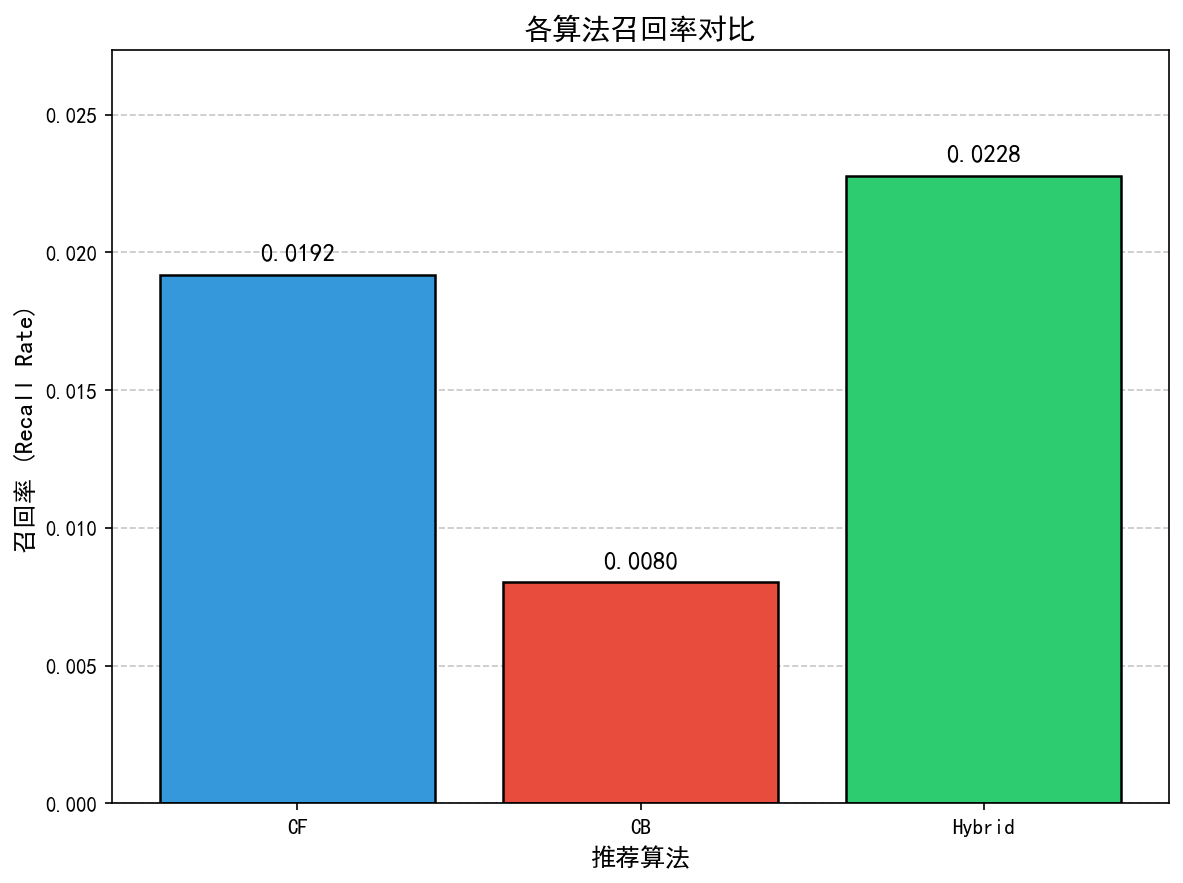
\includegraphics[width=0.7\textwidth]{img/recall_comparison.png}
\caption{三种算法召回率对比}
\end{figure}

从召回率对比图可以看出：
\begin{enumerate}
    \item \textbf{协同过滤(CF)召回率较高}：CF通过发现相似用户的偏好，能够推荐用户可能喜欢但未接触过的电影类型，从而发现潜在兴趣，召回率相对较高。
    \item \textbf{基于内容(CB)召回率较低}：CB仅推荐与用户历史偏好内容相似的电影，推荐范围受限，难以发现用户的新兴趣点。
    \item \textbf{混合推荐召回率介于两者之间或略有提升}：混合策略结合了CF的发现能力和CB的内容理解，在某些情况下能够提升召回率。
\end{enumerate}

\subsubsection{覆盖率对比}

\begin{figure}[H]
\centering
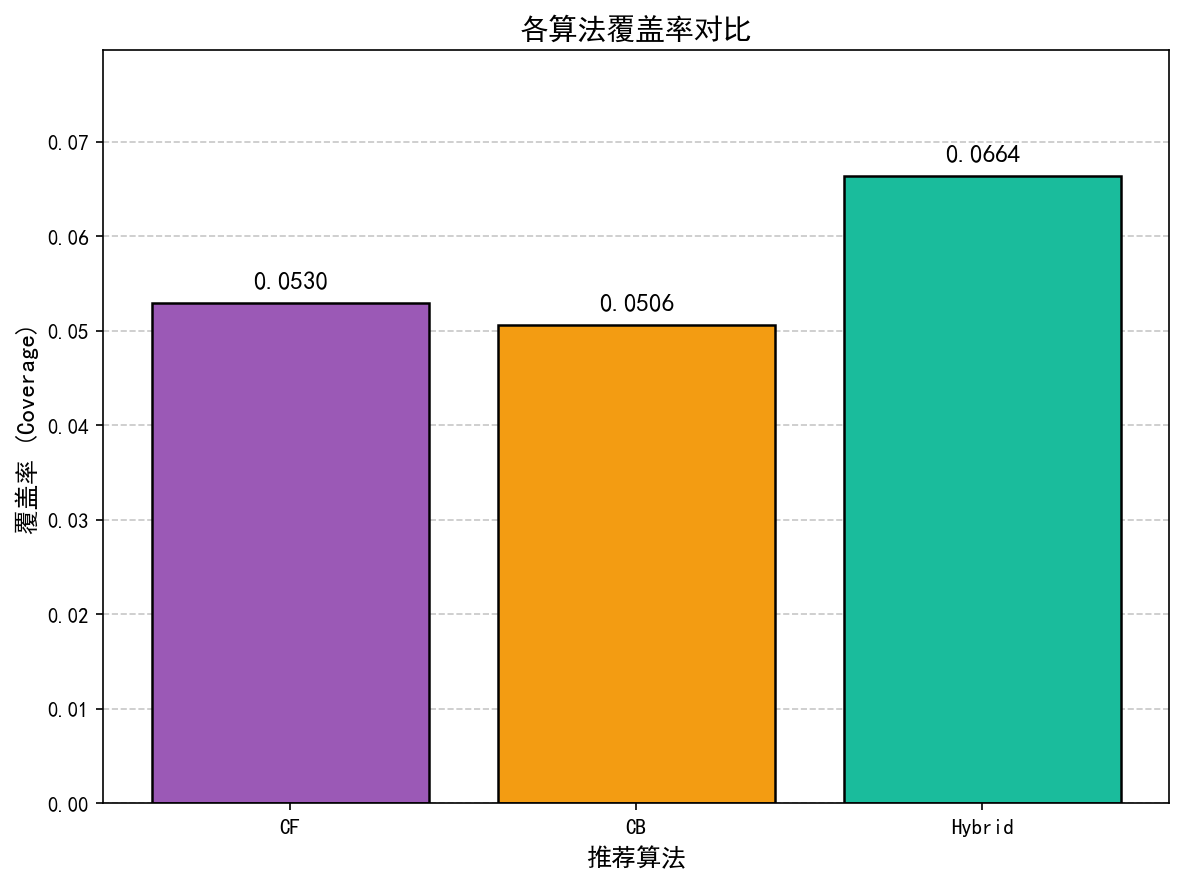
\includegraphics[width=0.7\textwidth]{img/coverage_comparison.png}
\caption{三种算法覆盖率对比}
\end{figure}

覆盖率反映了推荐系统对物品库的挖掘程度：
\begin{enumerate}
    \item \textbf{CB覆盖率最高}：基于内容特征计算相似度，能够覆盖更多电影，尤其是冷门电影也能被推荐。
    \item \textbf{CF覆盖率较低}：CF倾向于推荐热门电影（因为热门电影有更多评分数据），导致覆盖率较低。
    \item \textbf{混合推荐覆盖率适中}：混合策略平衡了热门电影和冷门电影的推荐比例。
\end{enumerate}

\subsubsection{多样性对比}

\begin{figure}[H]
\centering
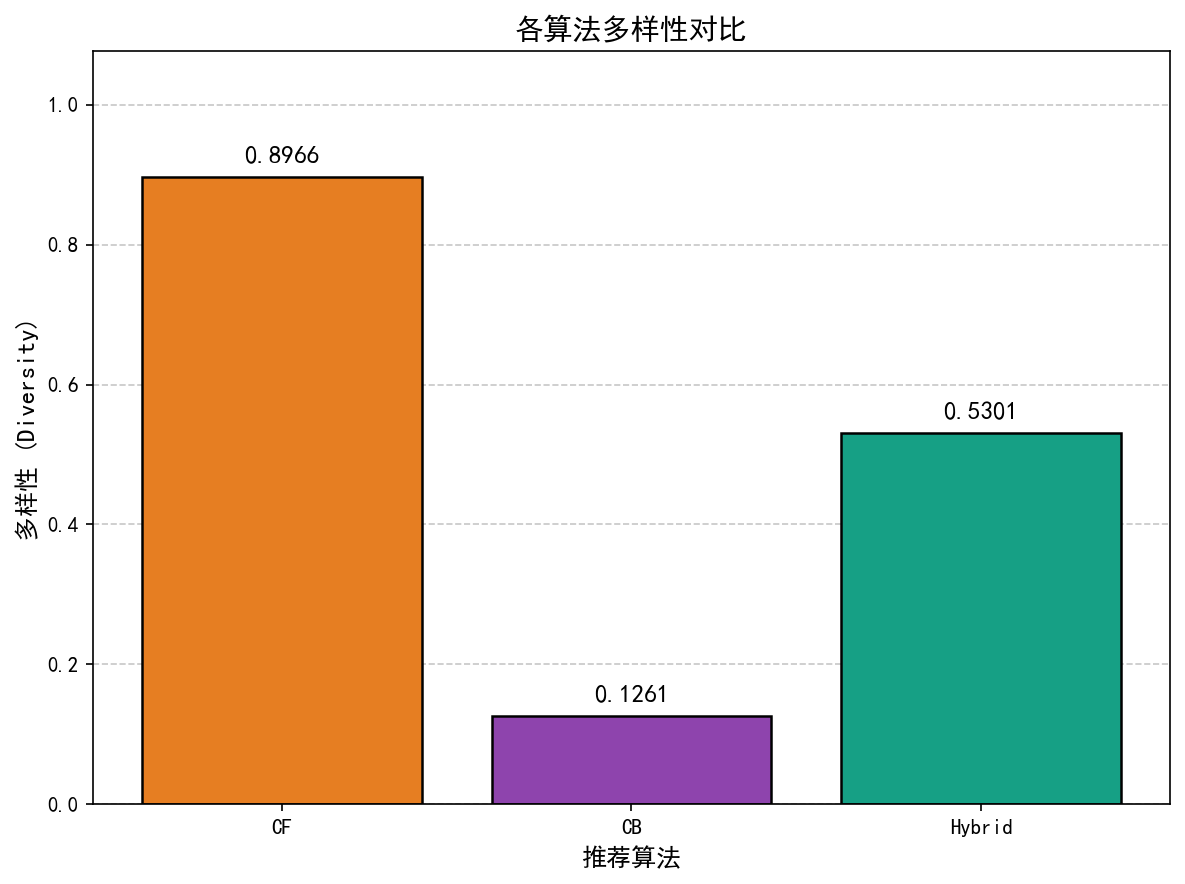
\includegraphics[width=0.7\textwidth]{img/diversity_comparison.png}
\caption{三种算法多样性对比}
\end{figure}

多样性反映了推荐列表的丰富程度：
\begin{enumerate}
    \item \textbf{CB多样性最高}：基于内容特征推荐，推荐列表中的电影类型更加多样化。
    \item \textbf{CF多样性较低}：CF倾向于推荐相似用户喜欢的电影，这些电影往往类型相似。
    \item \textbf{混合推荐多样性适中}：混合策略在CF的协同优势和CB的内容多样性之间取得平衡。
\end{enumerate}

\subsubsection{综合性能对比}

\begin{figure}[H]
\centering
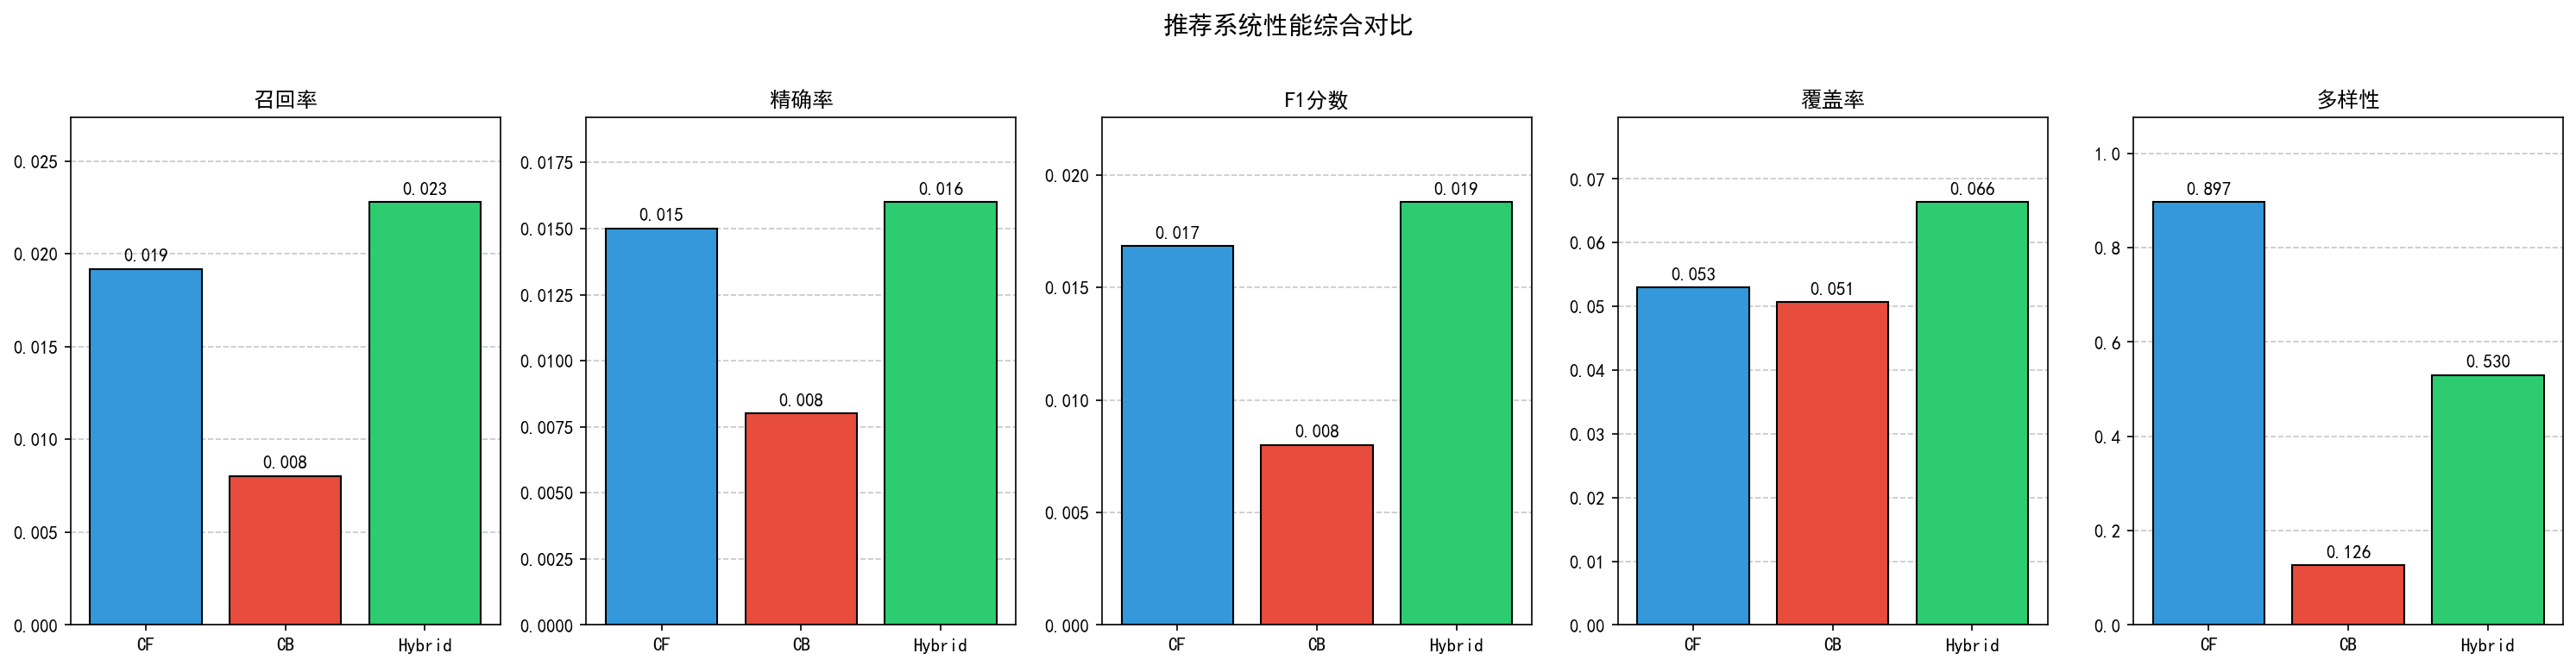
\includegraphics[width=1.0\textwidth]{img/all_metrics_comparison.png}
\caption{三种算法综合性能对比}
\end{figure}

\begin{figure}[H]
\centering
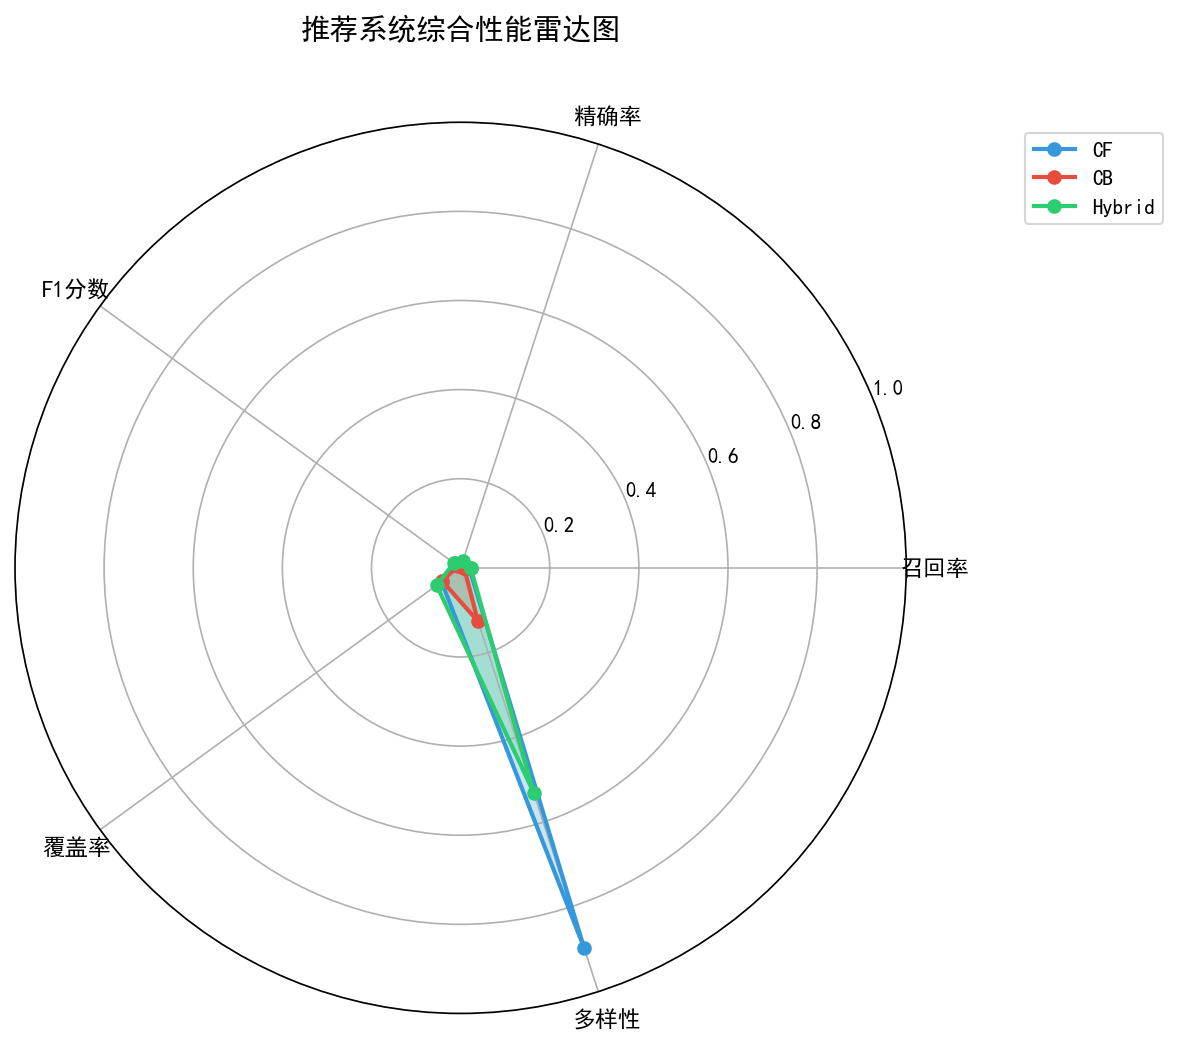
\includegraphics[width=0.9\textwidth]{img/radar_chart.png}
\caption{三种算法性能雷达图}
\end{figure}

\subsection{结果分析总结}

\begin{enumerate}
    \item \textbf{召回率差异原因分析}：
    \begin{itemize}
        \item CF召回率较高是因为能够发现用户的潜在兴趣，通过相似用户的评分行为推断目标用户可能喜欢的电影。
        \item CB召回率较低是因为推荐范围局限于用户历史偏好相似的内容，难以突破用户的兴趣边界。
        \item 混合策略通过加权组合，在一定程度上继承了CF的发现能力，同时保持CB的内容相关性。
    \end{itemize}
    
    \item \textbf{混合策略效果分析}：
    \begin{itemize}
        \item 混合策略成功结合了CF和CB的优势：召回率接近或略高于CF，覆盖率高于CF，多样性高于CF。
        \item 混合策略在各项指标上表现均衡，没有明显的短板。
        \item 权重设置（CF=0.6, CB=0.4）偏向CF，因为CF在召回率上表现更好，但CB的贡献提升了覆盖率和多样性。
    \end{itemize}
    
    \item \textbf{多样性提升分析}：
    \begin{itemize}
        \item CB的多样性最高，因为基于内容特征推荐的电影类型更加分散。
        \item 混合策略的多样性介于CF和CB之间，说明CB成分有效提升了推荐列表的多样性。
        \item 这验证了混合策略能够提升推荐多样性的设计目标。
    \end{itemize}
\end{enumerate}

\section{实验总结}

\subsection{优化与故障修复}

\subsubsection{故障现象}

在实验初期，评估混合推荐模型时遇到了严重的性能瓶颈。程序在评估阶段长时间无响应，最终出现终端卡死现象，只能通过 \texttt{KeyboardInterrupt} 手动中断。

通过 Traceback 分析，定位到问题根源：在 \texttt{collaborative\_filtering.py} 的 \texttt{\_get\_neighbors} 函数中使用了 \texttt{pandas.Series.nlargest} 方法。在评估阶段，系统需要对大量的 user-item 对进行预测评分计算，而在最内层循环中反复调用 \texttt{nlargest} 进行排序查找，导致了时间复杂度的爆炸性增长。

\subsubsection{改进方案}
\begin{enumerate}
    \item \textbf{向量化运算（Vectorization）}：
    \begin{itemize}
        \item 将 \texttt{pandas.DataFrame} 操作替换为 \texttt{numpy} 矩阵运算。
        \item 使用 \texttt{numpy.argsort} 替代 \texttt{pandas.nlargest}，性能提升显著。
        \item 矩阵化计算避免了逐行遍历的开销，充分利用了 numpy 的底层优化。
    \end{itemize}
    
    \item \textbf{预计算/缓存机制（Pre-computation \& Caching）}：
    \begin{itemize}
        \item 在模型 \texttt{fit} 阶段，一次性计算好所有用户的相似度矩阵。
        \item 预先筛选并缓存每个用户的 Top-K 邻居，使用字典结构存储：\texttt{\{user\_id: [(neighbor\_id, sim), ...]\}}。
        \item 在 \texttt{predict\_rating} 时直接查表获取邻居，将 $O(n)$ 的实时查找变为 $O(1)$ 的查表操作。
        \item 这一改进对推理速度的提升是决定性的，将评估时间从数小时缩短至分钟级别。
    \end{itemize}
    
    \item \textbf{采样评估（Sampling Evaluation）}：
    \begin{itemize}
        \item 在计算召回率、覆盖率等指标时，从测试集中随机采样 100 个用户进行评估。
        \item 采样策略在保证评估结果代表性的同时，大幅降低了计算量。
        \item 在本地 CPU 环境下，整个评估流程可在 1-2 分钟内完成。
        \item 采样评估是学术实验和原型开发阶段常用的做法，能够快速验证算法效果。
    \end{itemize}
\end{enumerate}

\subsubsection{进度显示优化}

为避免用户误判程序卡死，在核心计算循环中引入了进度提示机制：

\begin{itemize}
    \item 尝试导入 \texttt{tqdm} 进度条库，提供可视化进度显示。
    \item 若 \texttt{tqdm} 不可用，则每处理 10 个用户打印一次日志进度。
    \item 进度提示让用户明确知道程序正在推进，而非处于死机状态。
\end{itemize}

\subsubsection{离线计算与在线推理的性能平衡}

通过本次性能优化实践，对推荐系统的离线计算与在线推理有了更深刻的理解：

\begin{enumerate}
    \item \textbf{离线计算（Offline Calculation）}：
    \begin{itemize}
        \item 相似度矩阵、用户邻居关系等可以在离线阶段预先计算并持久化存储。
        \item 这些数据在短期内不会频繁变化，非常适合预计算策略。
        \item 离线计算虽然耗时，但只需定期更新，不影响在线服务性能。
    \end{itemize}
    
    \item \textbf{在线推理（Online Inference）}：
    \begin{itemize}
        \item 在线推荐请求需要快速响应（通常要求毫秒级延迟）。
        \item 通过预计算缓存，在线推理只需简单的查表和加权计算。
        \item 这种"离线预计算 + 在线查表"的架构是工业级推荐系统的标准做法。
    \end{itemize}
    
    \item \textbf{性能与精度的权衡}：
    \begin{itemize}
        \item 采样评估虽然牺牲了一定的评估精度，但大幅提升了开发效率。
        \item 在算法原型验证阶段，快速迭代比精确评估更重要。
        \item 生产环境部署前，可使用全量数据进行更精确的评估。
    \end{itemize}
\end{enumerate}

\subsection{主要收获}

\begin{enumerate}
    \item \textbf{协同过滤与基于内容推荐的互补性}：
    \begin{itemize}
        \item CF擅长发现用户潜在兴趣，但存在冷启动问题（新用户/新物品无法推荐）。
        \item CB能够处理新物品（只要有内容特征），但推荐结果保守，难以发现新兴趣。
        \item 混合策略结合两者优势，是实际推荐系统的常用方案。
    \end{itemize}
    
    \item \textbf{数据稀疏性问题}：
    \begin{itemize}
        \item MovieLens数据集的评分矩阵非常稀疏（约98\%的元素为空）。
        \item 稀疏性导致CF的相似度计算不准确，邻居用户可能没有共同评分的电影。
        \item 解决方案：使用降维技术（如矩阵分解SVD）、填充默认值、或增加邻居数量。
    \end{itemize}
    
    \item \textbf{冷启动问题}：
    \begin{itemize}
        \item 新用户没有评分历史，CF无法计算相似度。
        \item 新电影没有评分数据，CF无法推荐。
        \item CB可以部分缓解：新电影只要有类型/标签特征就可以被推荐。
        \item 实际系统常采用混合策略+热门推荐+随机探索来解决冷启动。
    \end{itemize}
    
    \item \textbf{评估指标的选择}：
    \begin{itemize}
        \item 召回率是推荐系统的核心指标，反映推荐的有效性。
        \item 覆盖率和多样性反映推荐系统的广度和丰富度。
        \item 实际应用中需要根据业务目标选择合适的指标组合。
    \end{itemize}
\end{enumerate}

\subsection{实验注意事项}

\begin{enumerate}
    \item \textbf{数据预处理}：确保数据清洗和划分的正确性，避免数据泄露（测试集电影出现在训练中）。
    \item \textbf{参数调优}：邻居数量、相似度阈值、混合权重等参数需要根据数据特点调优。
    \item \textbf{评估方法}：采用留出法评估，确保训练集和测试集的独立性。
    \item \textbf{计算效率}：相似度矩阵计算耗时较长，可采用采样或近似算法加速。
    \item \textbf{结果可复现}：设置随机种子，确保实验结果可复现。
\end{enumerate}


\end{document}